\section{Architecture}
\label{sec:introduction}

To instrument an application we use an execution wrapper. This wrapper instructs
the runtime linker to load our library tthread by setting \emph{LD\_PRELOAD}. It
also prepares a file, which is later on used by tthread to log the thread
schedule and data dependence graph during execution. To obtain control flow,
we use an new Intel ISA Extension, called Processor Trace (PT).
In Linux this processor feature is exposed to userland as a Perfomance Measuring
Unit (PMU) in the perf event interface.

The Perf interface on Linux consists of a syscall, which gives back a file
descriptor. Events are accessed by obtaining buffers via mmap(2) and can be
further controlled via ioctl syscalls on the given file descriptor. Along with
interface the userspace \emph{perf} allows to dump and filter from these
buffers. In the case of Inspector filtering is done by using Linux control
groups (Also known as Cgroups). Cgroups are a kernel feature to apply constraint
like resource usage to a group of processes. It has the property, that by
default every child process belongs to the same process as its parent. Also for
\emph{perf\_events} such a cgroup exists. The execution wrapper will create such
a croup exclusivly for the application under test. This is done because
\emph{tthread} will cause applications using threads to create multiple
processes instead, which process ids are not known it advance.

The subcommand \emph{perf record} is then used to dump the trace produced by PT.
Intel PT generates their for a stream of TNT packets, which denotes the
condional branches taken and TIP packets for indirect branches and function
returns. The data is referenced as a sample event in the perf event list and
stored in a ring buffer called \emph{AUX area}. If perf tool cannot
keep up with processor trace it is possible (for example an interrupt occurs),
theire will be gaps in the trace. PSB packets allow to resynchronize over these
gapps.

\begin{figure}[h]
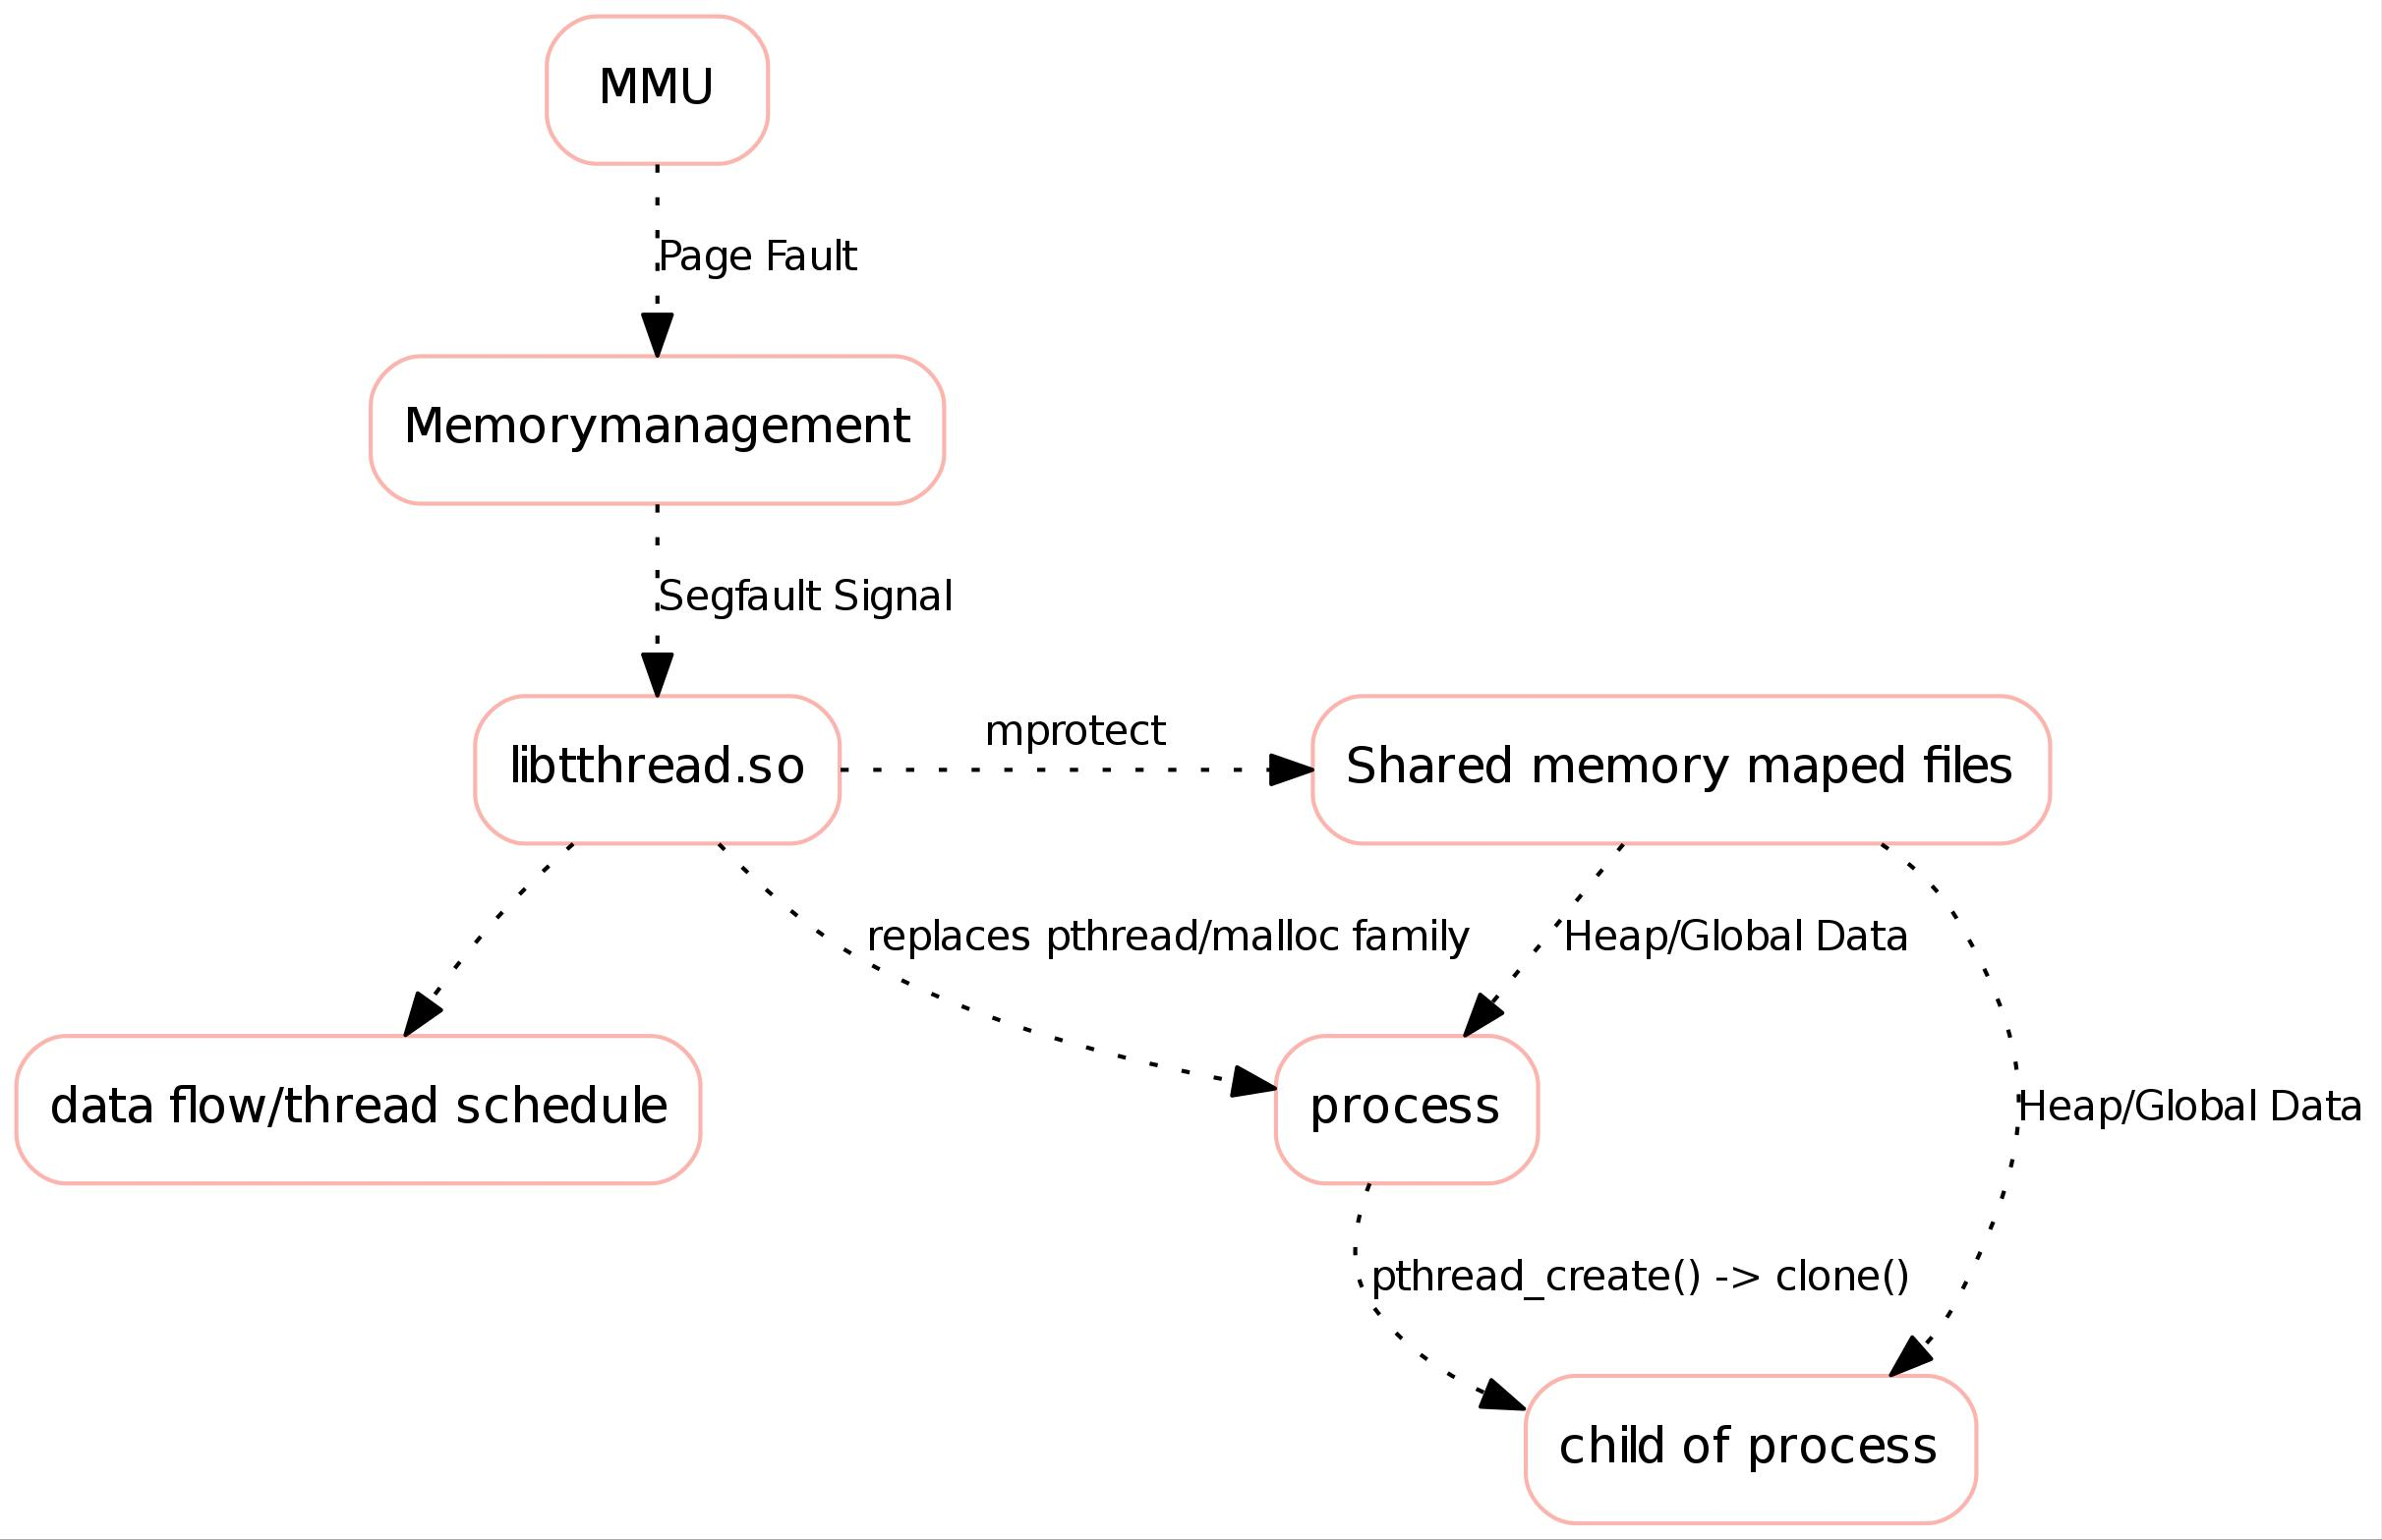
\includegraphics[width=8cm]{figure/arch.jpg}
\caption{Libtthread Architecture}
\label{fig:tthread}
\end{figure}

\begin{figure}[h]
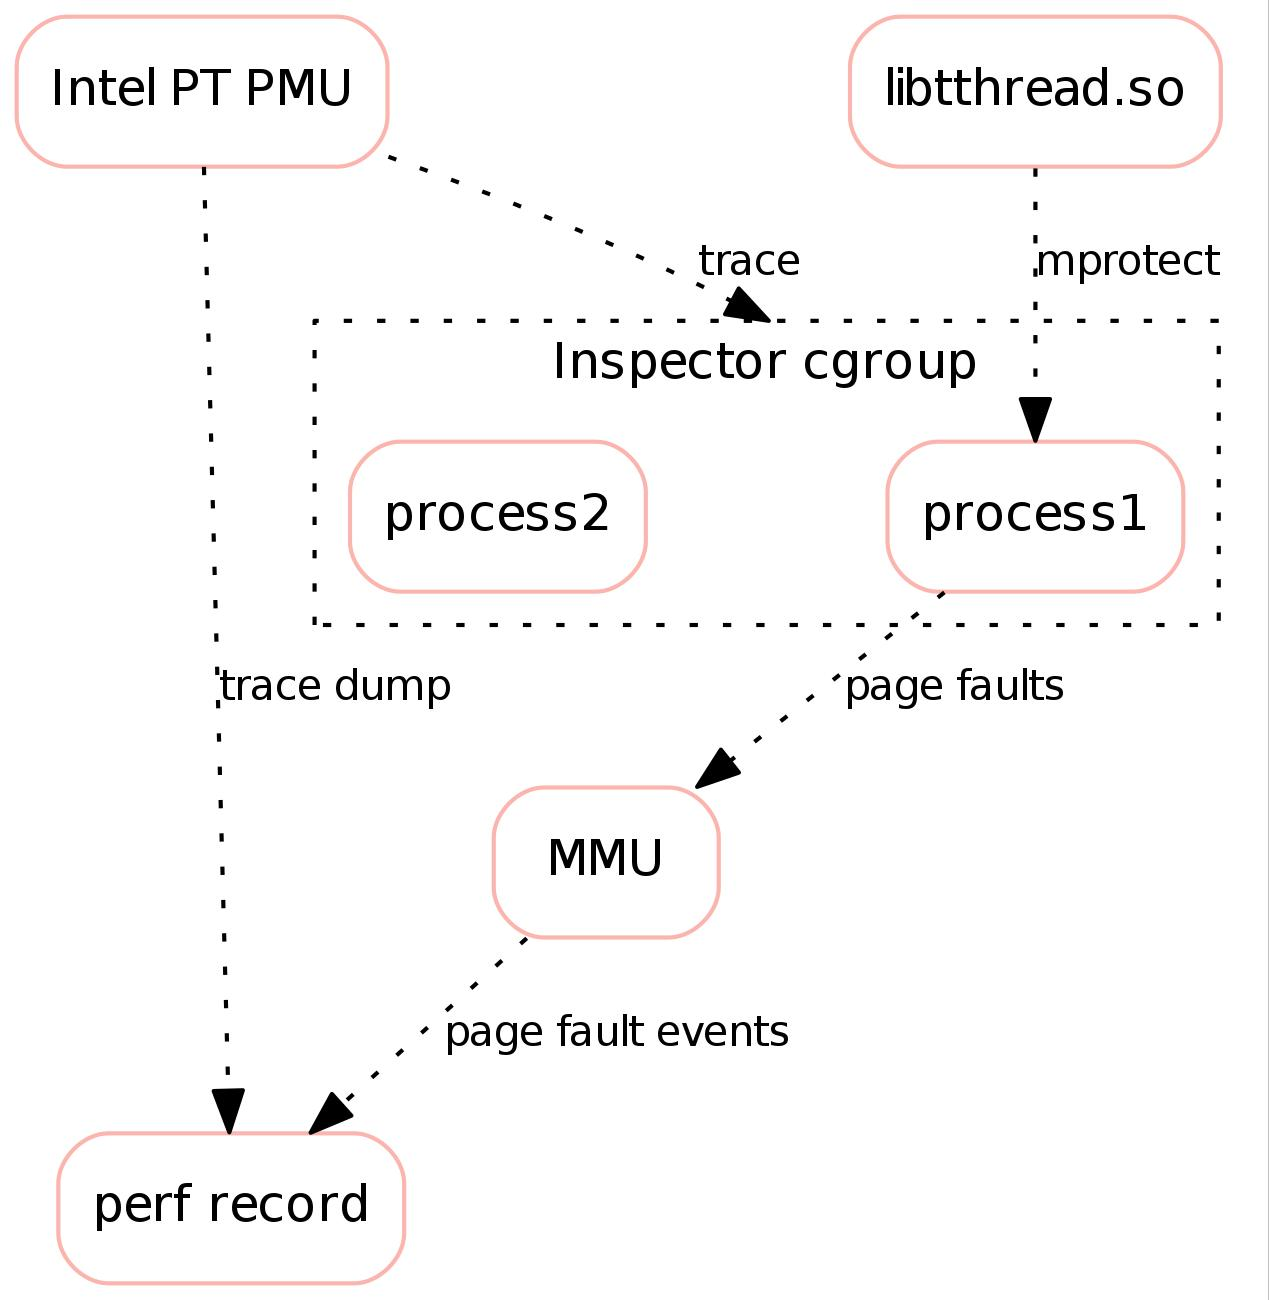
\includegraphics[width=8cm]{figure/arch2.jpg}
\caption{Inspector Architecture}
\label{fig:inspector}
\end{figure}

Along with PT page fault events generated by the kernel will be included
addionally to the trace packets. Because \emph{tthread} uses \emph{mprotect}
syscall to monitor access of heap and global memory space, whenever the
application access this memory, the MMU will generate page fault. These
page fault also includes the location, where in code memory was accessed.

After execution the result can be further processed by using a set of tools
for example \emph{perf script}. The branch information is still in a compressed
form and needs to be decoded. Perf has a decoder integrated to achieve this.
To map the trace onto binaries, it needs access to executables and linked
libraries of the application. During the excecution mmap events are tracked to
know to the location of each loadable.
